Nachdem der genaue Ablauf des Algorithmus erklärt wurde, bleibt die Frage: Wie oft muss die Grover Iteration durchgeführt werden, um mit einer hohen Wahrscheinlichkeit das gesuchte Element $\mathbf{\hat{x}}$ zu messen? noch offen.

\subsection{Geometrische Veranschaulichung}
Mithilfe von Regeln aus der Geometrie kann die Anzahl der Iterationen bestimmt werden. Das Schrittweise erhöhen der Amplitude des gesuchten Elements kann auf der Bloch Kugel als Rotation aufgefasst werden. 
\\
In der Geometrie entspricht die Spiegelung eines Punktes an zwei Ebenen eine Drehung um den Winkel $\mathbf{2 \times \beta}$, wobei $\mathbf{\beta}$ der Winkel zwischen den Ebenen ist. Dies ist in der Abbildung \ref{fig:zweiEbenen} verdeutlicht. Diese Eigenschaft kann sich zunutze gemacht werden. Ist der Winkel bekannt, kann ausrechnet werden, um wie viel der Grad gedreht werden muss, um das gesuchte Element zu erreichen und damit wie oft die Grover-Iteration durchgeführt werden muss.
 \begin{figure}[hbtp]
	\centering
	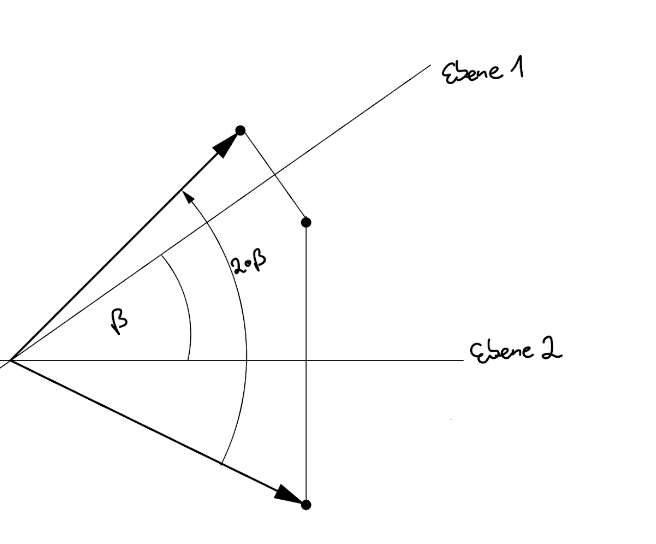
\includegraphics[width=.6\textwidth]{figures/zweiEbenen.png}
	\caption{$\mathbf{R_4}$ Spiegelung an zwei Ebenen \\ Quelle: Anlehnung an \cite[S. 149]{Ho17}}
	\label{fig:zweiEbenen}
\end{figure} 
\noindent
\\
Wie der Name schon sagt, handelt es sich bei der Spiegelung am Mittelwert um eine Spiegelung. Die zweite Spiegelung ist das negieren von dem gesuchten Element $\mathbf{\hat{x}}$. Die Formel zur Spiegelung an einem Wert $\mathbf{m}$ lautet: $\mathbf{\alpha \rightarrow 2 \times m - \alpha}$. Ist $\mathbf{m=0}$ erhalten wir $\mathbf{\alpha \rightarrow - \alpha}$. Dies zeigt, dass die Negation eines Elementes eine Spiegelung an dem Wert $\mathbf{0}$ ist.
\\ 
\\
Der Winkel lautet $\mathbf{\sin(\beta) = \langle s | \hat{x} \rangle}$, mit $\mathbf{s = \frac{1}{\sqrt{N}}\sum\limits_{x=0}^{N-1}|x\rangle}$, welches die Allgemeine Superposition ist. Ausrechnet ergibt dies $\mathbf{\sin(\beta) = \frac{1}{\sqrt N}}$. Daran lässt sich erkennen, dass die Anzahl der Iterationen abhängig von der Anzahl der Datenbankelemente ist und nicht von $\mathbf{\hat{x}}$. Wäre dies nicht so, hätte das zur Folge, dass für jedes gesuchte Element die Anzahl der Grover Iterationen angepasst werden müsste.
\subsubsection{Beispielrechnung: Geometrische Veranschaulichung}
Sei $\mathbf{N=4}$, dann folgt daraus, dass $\mathbf{\sin(\beta) = \frac{1}{\sqrt{4}}}$ ist. Nach Beta aufgelöst ergibt sich $\mathbf{\beta = \frac{\pi}{6}}$.
\\
Wird nun eine Grover Iteration durchgeführt, ändert sich der Winkel wie folgt: $\mathbf{\beta = \frac{\pi}{6} + 2 \times \frac{\pi}{6}  = \frac{\pi}{2}}$. Wird nun $\mathbf{sin(\frac{\pi}{2}))}$ ausgerechnet, erhalten wir $\mathbf{1}$. Dies bedeutet, dass wir mit einer Drehung das gesuchte Element erreicht haben. Wird nun gemessen, erhalten wir mit einer Wahrscheinlichkeit von 100 \% das gesuchte Element. Dies wird auch wie im Abschnitt  \ref{sec:spiegelnAmMittelwert}  beschrieben erwartet.

\subsubsection{Anzahl an Grover Iterationen}
Durch die Rechnung konnte gezeigt werden, dass der Startwinkel $\mathbf{\frac{1}{\sqrt{N}}}$ beträgt und der Winkel nach $\mathbf{T}$ Grover Iterationen der Winkel den Wert $\mathbf{(2 \times T + 1)\times \frac{1}{\sqrt{N}}}$ hat. 
Falls für $\mathbf{T = \frac{\pi}{4}\times \sqrt{N}}$ gewählt wird, wird immer sehr nah an das gesuchte Element rotiert. 
\\
In der praktischen Umsetzung muss $\mathbf{T}$ immer abgerundet werden, da nur eine gerade Zahl an Iterationen durchgeführt werden kann. Wird $\mathbf{T}$ aufgerundet, werden zu viele Grover-Iterationen durchgeführt und es wird sich vom gesuchten Element wieder entfernt. \cite[S. 157]{KLM07} Das Souffl\'{e} würde anfangen einzugehen
\\
\\
Dadurch, dass die Anzahl der Grover-Iterationen $\mathbf{ \frac{\pi}{4}\times \sqrt{N}}$ beträgt und in jeder Iteration einmal das Quantenorakel aufgerufen wird, beträgt die Laufzeit des Grover Algorithmus $\mathbf{O(\sqrt N)}$.
